\documentclass{article}

\usepackage{hyperref}


\usepackage{pgf}
\usepackage{tikz}
\usetikzlibrary{arrows,shapes,snakes,automata,backgrounds,petri,matrix}

\author{John Lee \\ me@qinka.pro \\ qinka@live.com}
\title{A Figure for Nao-classify-server's Neural Network}

\begin{document}
    \maketitle
    A figure for nao-classify-server's neural network.
    \begin{figure}
        \centering
        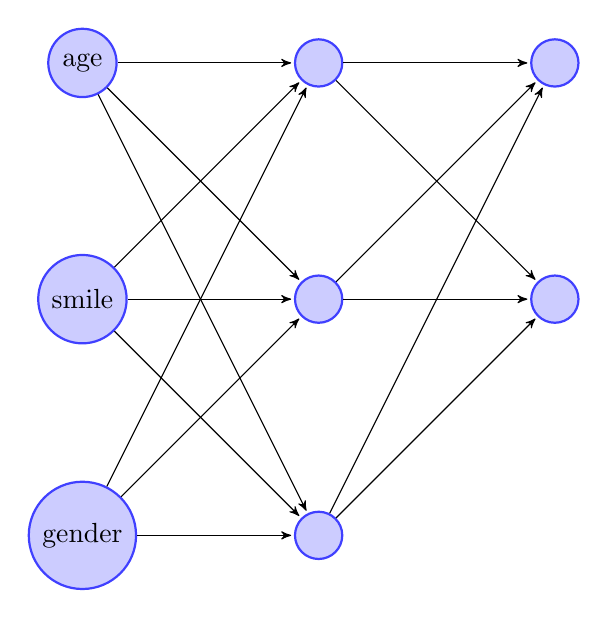
\begin{tikzpicture}[node distance=3cm,>=stealth',bend angle=20,auto]        
            \tikzstyle{point}=[circle,thick,draw=blue!75,fill=blue!20,minimum size=6mm]
            \begin{scope}
            \node[point](age){age};
            \node[point,below of=age](smile){smile};
            \node[point,below of=smile](gender){gender};
            \node[point,right of=age](h1){}
                edge [pre] node {} (age)
                edge [pre] node {} (smile)
                edge [pre] node {} (gender);
            \node[point,below of=h1](h2){}
                edge [pre] node {} (age)
                edge [pre] node {} (smile)
                edge [pre] node {} (gender);
            \node[point,below of=h2](h3){}
                edge [pre] node {} (age)
                edge [pre] node {} (smile)
                edge [pre] node {} (gender);
            \node[point,right of=h1](y1){}
                edge [pre] node {} (h1)
                edge [pre] node {} (h2)
                edge [pre] node {} (h3);
            \node[point,right of=h2](y2){}
                edge [pre] node {} (h1)
                edge [pre] node {} (h2)
                edge [pre] node {} (h3);
            \end{scope}
        \end{tikzpicture}
        \caption{Neural Network}
        \label{fig:nn}
    \end{figure}
\end{document}